\subsection{Stazionarietà}
In questo sottocapitolo verrà spiegato il concetto di stazionarietà di una serie
temporale e come poter capire se la serie interessata sia stazionaria.
 
\paragraph{Stazionarietà di una serie temporale} %TODO: citare http://www.seanabu.com/2016/03/22/time-series-seasonal-ARIMA-model-in-python/
Per essere stazionaria una serie temporale deve soddisfare
una lista di requisiti:
\begin{enumerate}
    
    \item \textbf{Media costante nel tempo}: La media della serie non deve essere 
    una funzione del tempo. Il grafico rosso, in figura~\ref*{fig:nons_mean}, non è stazionario 
    perché la media aumenta nel tempo~\cite{sa:stationary}.

    \begin{figure}[H]
        \centering
        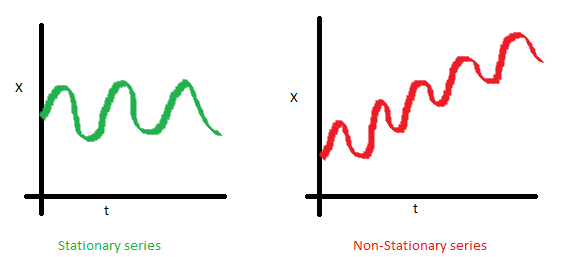
\includegraphics[width=0.65\linewidth,keepaspectratio]{nonstationary_mean.png}
        \caption{Media non costante nel tempo.}
        \label{fig:nons_mean}
    \end{figure}


    \item \textbf{Varianza costante nel tempo}: La varianza della serie non deve 
    essere funzione del tempo. Questa proprietà è nota come omoscedasticità. 
    Nel grafico rosso, in figura~\ref*{fig:nons_var}, 
    si noti la variazione della varianza dei dati nel tempo~\cite{sa:stationary}.

    \begin{figure}[H]
        \centering
        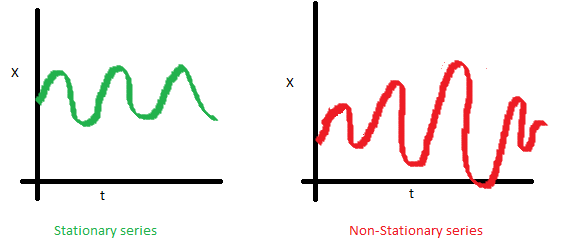
\includegraphics[width=0.65\linewidth,keepaspectratio]{nonstationary_variance.png}
        \caption{Varianza non costante nel tempo.}
        \label{fig:nons_var}
    \end{figure}

    \item \textbf{Covarianza costante nel tempo}: Infine, la covarianza del 
    termine $i$ e del termine $(i + m)$ non deve essere funzione del tempo. 
    Nel grafico, in figura~\ref*{fig:nons_cov}, si può notare che lo spread 
    diventa più vicino all'aumentare del tempo. Pertanto, 
    la covarianza non è costante nel tempo per la ``serie rossa''~\cite{sa:stationary}.

    \begin{figure}[H]
        \centering
        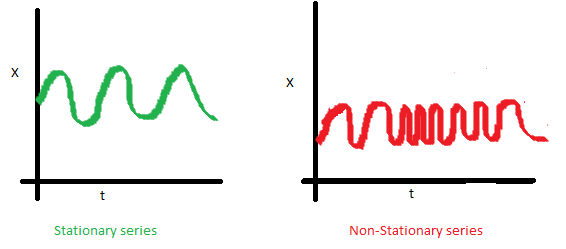
\includegraphics[width=0.65\linewidth,keepaspectratio]{nonstationary_cov.png}
        \caption{Coviarianza non costante nel tempo.}
        \label{fig:nons_cov}
    \end{figure}

    Per capire meglio il concetto di covarianza costante nel tempo 
    consideriamo una sequanza di variabili casuali, esse si definiscono
    con stazionarietà debole o stazionarietà della covarianza se:

    \begin{itemize}
        \setlength\itemsep{-0.6em}
        \item Tutti i termini della sequenza hanno la stessa media.
        \item La covarianza tra due termini qualsiasi della sequenza 
        dipende solo dalla posizione relativa dei due termini e non dalla 
        loro posizione assoluta.
    \end{itemize}

    Per posizione relativa di due termini si intende la distanza che 
    li separa l'uno dall'altro nella sequenza mentre per posizione assoluta, 
    si riferisce al punto in cui si trovano nella sequenza~\cite{sl:cov_stat}.

    \begin{figure}[H]
        \centering
        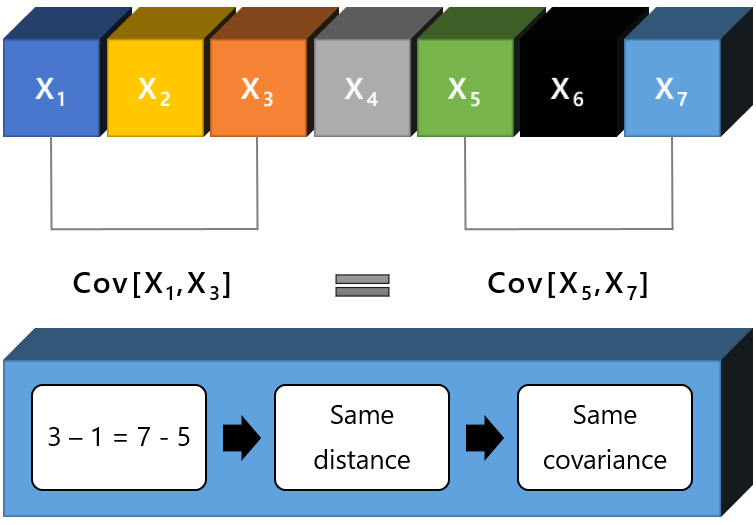
\includegraphics[width=0.4\linewidth,keepaspectratio]{stationary_cov.png}
        \caption{Stazionarietà della covarianza.}
    \end{figure}

\end{enumerate}


\subsubsection{Dickey Fuller Test}